%\documentclass[xcolor=dvipsnames,compress,handout]{beamer}
\documentclass[xcolor=dvipsnames,compress]{beamer}
\usepackage[utf8]{inputenc}
\usepackage[ngerman,english]{babel}
\usepackage{pgf}
\usepackage{graphicx}
\graphicspath{ {images/} }
\usepackage[absolute,overlay]{textpos}
\usepackage{xcolor}
\usepackage{comment}
%\usepackage{algorithm2e}
%\usepackage{algorithmic}
\usepackage{xpatch}
\usepackage{tabularx}
\usepackage[export]{adjustbox}
\usepackage{tikz}
\usepackage{pgffor}
\usepackage{blindtext}

% DESIGN
\definecolor{RUBblue}{rgb}{0,0.21,0.38}
\definecolor{AIblue}{rgb}{0,0.57,0.87}

% DO NOT ASK WHAT HAPPENS HERE
% Okay...
\useoutertheme[subsection=false]{miniframes}
\usecolortheme{beaver}
\beamertemplatenavigationsymbolsempty
\setbeamertemplate{footline}{%
    \begin{beamercolorbox}[wd=\paperwidth,ht=0ex,left]{default}
        %\insertauthor\hfill\insertframenumber%
        \colorbox{AIblue}{\vphantom{2cm}\hspace{14cm}}
    \end{beamercolorbox}
}
\setbeamercolor{item}{fg=RUBblue}
\setbeamercolor{title}{fg=Black}
\setbeamercolor{frametitle}{fg=Black}
\setbeamerfont{title}{size=\large}
\setbeamertemplate{itemize items}[square]
\setbeamercolor{section in head/foot}{bg=AIblue}
\setbeamerfont{footline}{size=\fontsize{15}{12}\selectfont}


\xpatchcmd{\itemize}
  {\def\makelabel}
  {\setlength{\itemsep}{0.2cm}\def\makelabel}{}{}

 
\addtobeamertemplate{frametitle}{}{%
\begin{textblock*}{100mm}(1.05\textwidth,0.535cm)

\includegraphics[height=0.975cm,width=0.98cm]{logo-rub.png}
\end{textblock*}}

% COMMANDS
\newcommand\NEWLINECOMMENT[1]{\STATE\STATE/* #1 */}
\newcommand\Only[2]{\only<#1|handout:#1>{#2}}
\newcommand\overlayImage[6]{
	\only<#1|handout:#2>{
		\begin{textblock*}{\textwidth}(#3cm,#4cm)
			\frame{
				\includegraphics[width=#5\textwidth]{#6}
			}
		\end{textblock*}
	}
}


% TITLEPAGE
\title{\textbf{Deep Convolutional Networks}}
\author{Christian Andreas Mielers\\Phil Yannick Schrör}
\institute{Ruhr-University Bochum\\Institute for Neural Computation\\Study Project}
\date{24th of February 2016}
 
\begin{document}
\section{Welcome}
\subsection{Welcome}
\maketitle

\section{Convolutional Neural Networks}
\subsection{Convolutional Neural Networks}

\frame{
	\frametitle{Convolutional Neural Networks}
	\begin{columns}
		\column{0.5\textwidth}
			\begin{itemize}
				\item Learns the weights of convolutional filters
				\item Exploits spatial structure in the input
				\item Convolving entire input with filter implies shared weights
				\item Reduced amount of weights allows lots of filters
				\item Filters specific to color channels
			\end{itemize}
		\column{0.5\textwidth}
			\includegraphics<1>[width=\textwidth]{dense_layer}
			\includegraphics<2>[width=\textwidth]{convolutional_layer}
			\includegraphics<3>[width=\textwidth]{color_mapping}
	\end{columns}
}

\frame{
	\frametitle{Network Structure}
	\begin{textblock*}{1.1\textwidth}(0.5cm,2.9cm)
		\footnotesize{
			\begin{tabularx}{\textwidth}{cp{0.16\linewidth}p{0.4\linewidth}X}
			\textbf{Layer} & \textbf{Type} & \textbf{Configuration} & \textbf{Activation function} \\
			& & & \\
			\hline
			& & & \\
			0 & Convolutional & 100 filters of size $7\times7$ per channel & $\tanh$ \\
			1 & Max Pooling & Pool size $2\times2$ & - \\
			2 & Convolutional & 150 filters of size $4\times4$ per channel & $\tanh$ \\
			3 & Max Pooling & Pool size $2\times2$ & - \\
			4 & Convolutional & 250 filters of size $4\times4$ per channel & $\tanh$ \\
			5 & Max Pooling & Pool size $2\times2$ & - \\
			6 & Dense & 300 neurons & $\tanh$ \\
			7 & Dense & 43 neurons & softmax
			\end{tabularx}
		}
		%TODO Add image of tanh function somewhere
	\end{textblock*}
}

\section{GTSRB}
\subsection{GTSRB}

\frame{
	\frametitle{German Traffic Sign Recognition Benchmark}
	\begin{columns}
		\column{0.5\textwidth}
			\begin{itemize}
				\item Dataset of traffic signs taken while on the road
				\item 39209 training and 12630 test images in 43 classes
				\item Images contain a 10\% border around the sign
				\item Annotations provide precise sign locations
					\begin{itemize}
						\item We cropped out just the sign
					\end{itemize}
			\end{itemize}
		\column{0.5\textwidth}
			\centering
			\includegraphics<1>[width=0.4\textwidth]{gtsrb_00002_00029}
			\includegraphics<2>[width=0.4\textwidth]{gtsrb_00002_00029_border}
			
			\includegraphics<1>[width=0.4\textwidth]{gtsrb_00013_00029}
			\includegraphics<2>[width=0.4\textwidth]{gtsrb_00013_00029_border}
			
			\includegraphics<1>[width=0.4\textwidth]{gtsrb_00029_00029}
			\includegraphics<2>[width=0.4\textwidth]{gtsrb_00029_00029_border}
	\end{columns}
	
	%TODO Maybe create three different plots: the first one shows only the results of the simple setup, the second adds the ones with distortions and the third adds the results, which we achieved by using the RELU activation function
	% Will do that
}

% TODO not finished yet, more like notes for myself
\frame{
	\frametitle{Simple Setup}
	\begin{itemize}
		\item Input size $48 \times 48$
		\item Contrast normalization
		\item Describe Simple Setup
		\item Present Results
	\end{itemize}
}

\begin{frame}
	\frametitle{Results on GTSRB}
	\begin{figure}
		\centering
		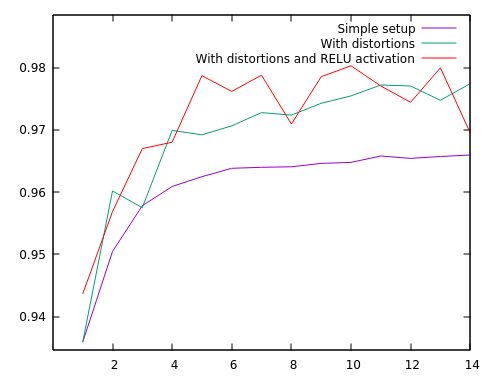
\includegraphics[width=0.85\textwidth]{gtsrb_results.png}
	\end{figure}
\end{frame}

\frame{
	\frametitle{Input Distortions}
	\begin{itemize}
		\item Mention input distortions
		\item Explain them
		\item Present distortion parameters
		\item Maybe add one or two images before and after the transformations
	\end{itemize}
}

\frame{
	\frametitle{Results with RELU}
	\begin{itemize}
		\item Add RELU image
		\item Present results with RELU activation function
	\end{itemize}
}

\frame[<+->]{
	\frametitle{Missclassified images}
	\begin{figure}
		\centering
		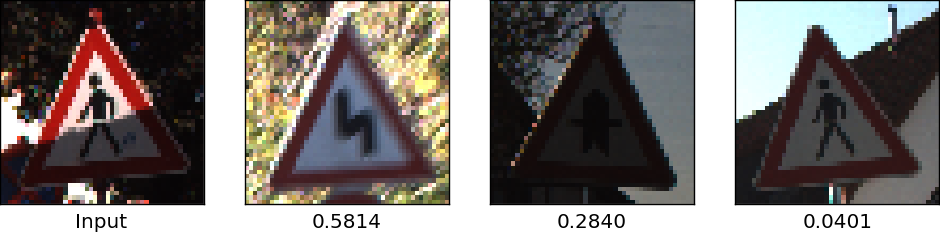
\includegraphics[width=0.85\textwidth]{gtsrb_mistakes/mistake_fussgaenger.png}\\
		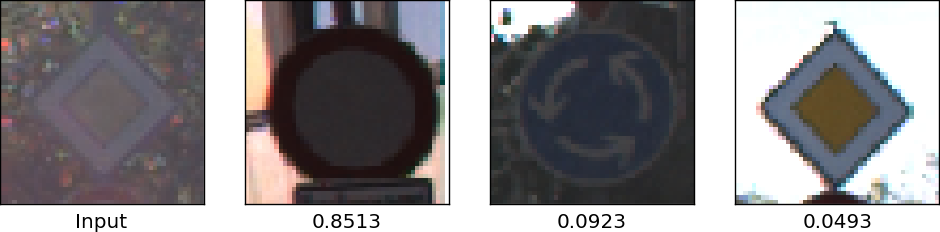
\includegraphics[width=0.85\textwidth]{gtsrb_mistakes/mistake_vorfahrtstrasse.png}\\
		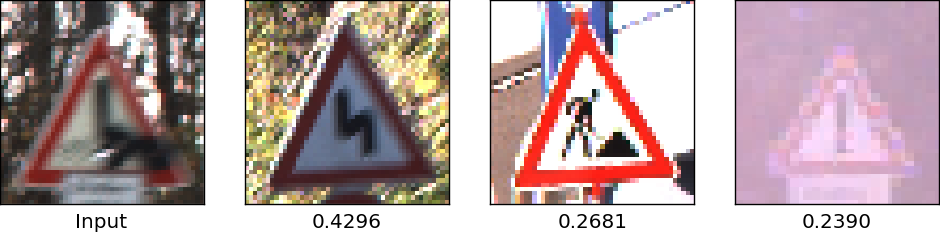
\includegraphics[width=0.85\textwidth]{gtsrb_mistakes/mistake_gefahrenstelle.png}
	\end{figure}
	%TODO Maybe choose more significant images
}

\section{Filter Reuse}
\subsection{Filter Reuse}

\frame{
	\frametitle{Filter Reuse}
	\begin{itemize}
		\item How well do the GTSRB filters generalize?
		\item Initialize new network with same structure randomly
		\item Copy GTSRB filters to the new network
		\item Train only the fully connected layers!
	\end{itemize}
}

\frame{
	\frametitle{COIL100}
	\begin{textblock*}{1.09\textwidth}(0.5cm,1.6cm)
		\begin{figure}
			\centering
			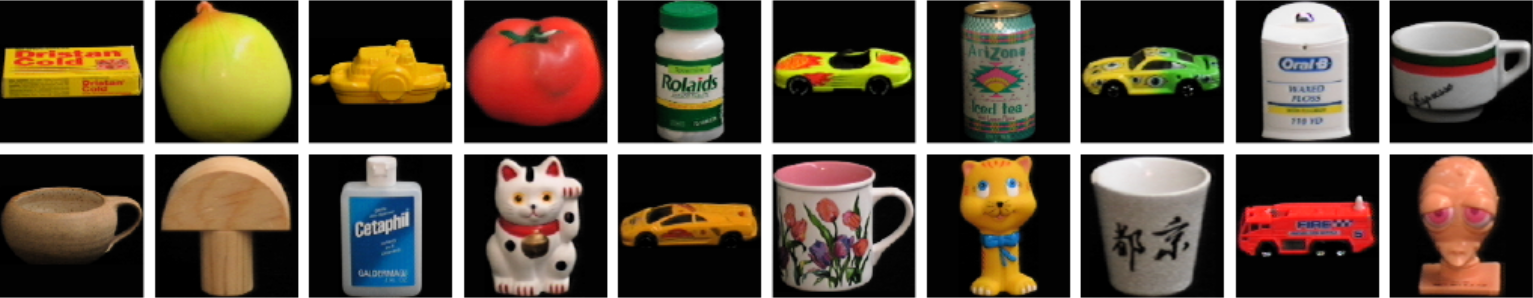
\includegraphics[width=\textwidth]{coil100.png}
		\end{figure}
	\end{textblock*}
	\begin{textblock*}{1.1\textwidth}(0.5cm,4.55cm)
		\begin{itemize}
			\item Columbia Object Image Library 100 $\Rightarrow$ COIL100
			\item 100 different objects
			\item Objects turning on a black turntable
			\item One photo each time the object has turned by $5^\circ$
			\item 72 images per object, 7200 images in total
			\item Random separation into 58 training and 14 test images per object
		\end{itemize}
	\end{textblock*}
}

\frame{
	\frametitle{COIL100 --- GTSRB Filters Results}
	\begin{textblock*}{1.1\textwidth}(0.3cm,1.1cm)
		\begin{figure}
			\centering
			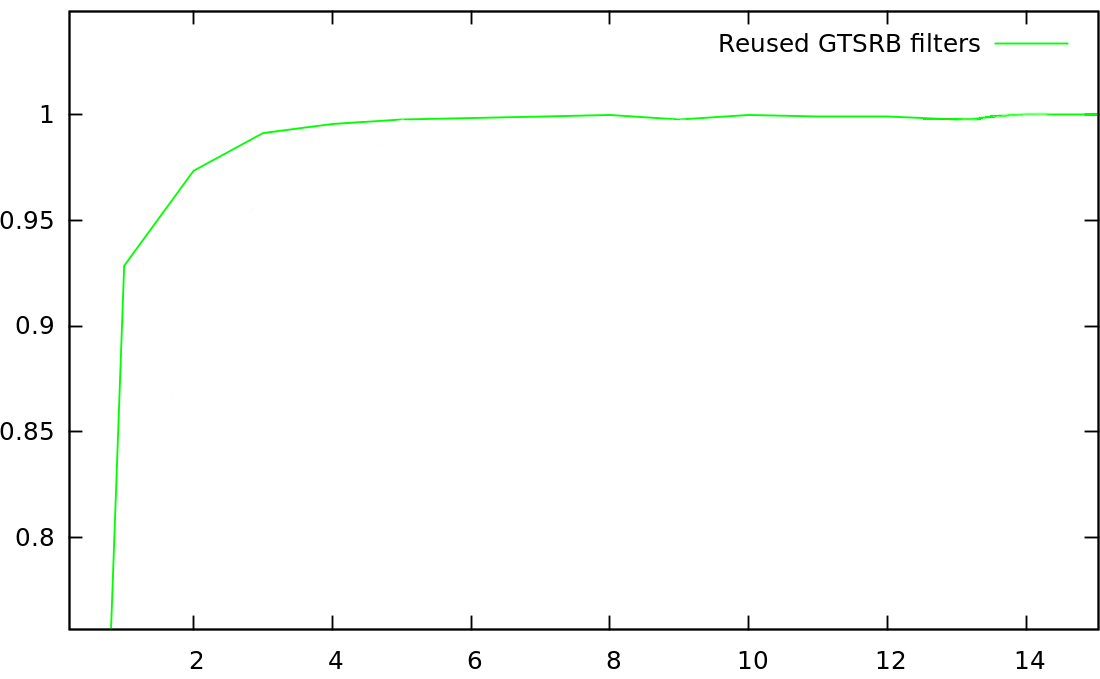
\includegraphics[width=1.02\textwidth]{coil100_results_gtsrb_only.png}
		\end{figure}
	\end{textblock*}
	\begin{textblock*}{1.1\textwidth}(1.8cm,4.5cm)
		\begin{itemize}
			\item Monotonic increase until the 8th epoch
			\item Random distortions $\Rightarrow$ Slight decreases
			\item One epoch takes around 5 minutes
			\item Good results in a short time
		\end{itemize}
	\end{textblock*}
	\begin{textblock*}{1.1\textwidth}(9.4cm,2.93cm)
		\scriptsize
		\begin{tabular}{|r|r|}
			\hline
			Epoch & Accuracy\\ \hline
			1 & 0.9286\\
			2 & 0.9736\\
			3 & 0.9914\\
			4 & 0.9957\\
			5 & 0.9979\\
			6 & 0.9986\\
			7 & 0.9993\\
			8 & 1.0000\\
			9 & 0.9979\\
			10 & 1.0000\\
			11 & 0.9993\\
			12 & 0.9993\\
			13 & 0.9979\\
			14 & 1.0000\\
			15 & 1.0000\\ \hline
		\end{tabular}
	\end{textblock*}
}

\frame{
	\frametitle{COIL100 --- Original filters}
	\begin{itemize}
		\item Which advantages does this approach have?
		\item We need data for a comparison
		\item Train a new network conventionally on COIL100
		\item Call the filters \emph{original}, which are created this way
		\item Compare training time and results!
	\end{itemize}
}


\frame{
	\frametitle{COIL100 --- Original Filters Results}
	\begin{textblock*}{1.1\textwidth}(0.3cm,1.1cm)
		\begin{figure}
			\centering
			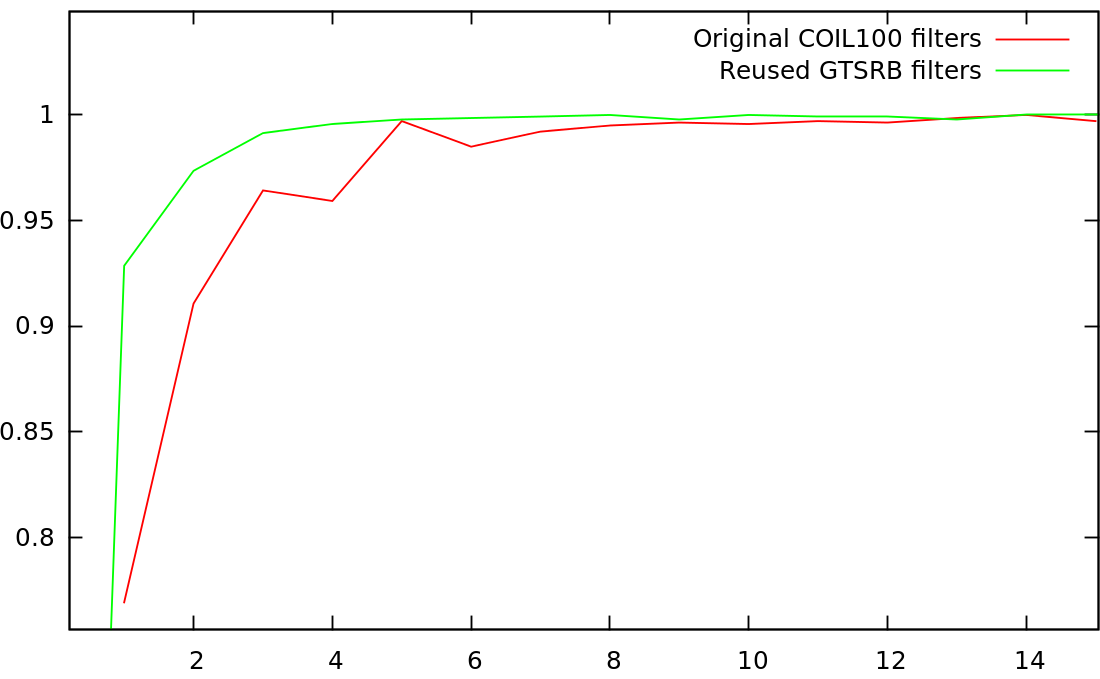
\includegraphics[width=1.02\textwidth]{coil100_results.png}
		\end{figure}
	\end{textblock*}
	\begin{textblock*}{0.5\textwidth}(2.8cm,4.5cm)
		\begin{itemize}
			\item GTSRB filters dominate
			\item Similar results in the end
			\item Training time: $\sim$ 90m
			\item How do the original filters look like?
		\end{itemize}
	\end{textblock*}
	\begin{textblock*}{1.1\textwidth}(8.2cm,2.945cm)
		\scriptsize
		\begin{tabular}{|r|rr|}
			\hline
			Epoch & GTSRB & Original\\ \hline
			1 & 0.9286 & 0.7693\\
			2 & 0.9736 & 0.9107\\
			3 & 0.9914 & 0.9643\\
			4 & 0.9957 & 0.9593\\
			5 & 0.9979 & 0.9971\\
			6 & 0.9986 & 0.9850\\
			7 & 0.9993 & 0.9921\\
			8 & 1.0000 & 0.9950\\
			9 & 0.9979 & 0.9964\\
			10 & 1.0000 & 0.9957\\
			11 & 0.9993 & 0.9971\\
			12 & 0.9993 & 0.9964\\
			13 & 0.9979 & 0.9986\\
			14 & 1.0000 & 1.0000\\
			15 & 1.0000 & 0.9971\\ \hline
		\end{tabular}
	\end{textblock*}
}

\frame{
	\frametitle{COIL100 --- How do the original filters look like?}
	\begin{textblock*}{1.1\textwidth}(0.3cm,1.3cm)
		\begin{figure}
			\centering
			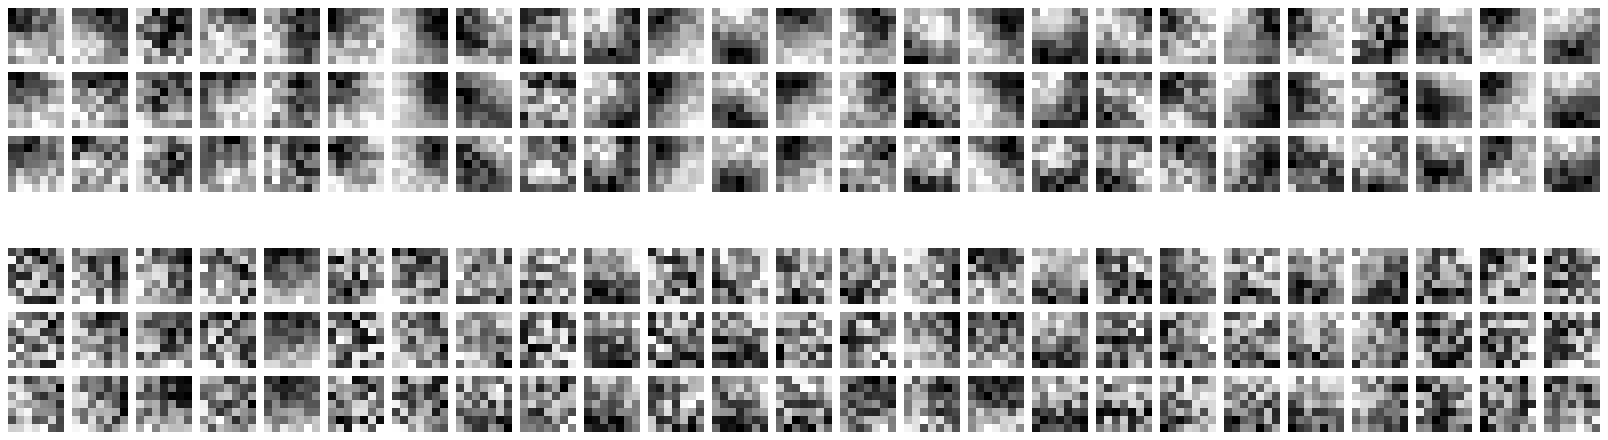
\includegraphics[width=1.03\textwidth]{gtsrb_vs_coil_filters.png}
		\end{figure}
	\end{textblock*}
	\begin{textblock*}{1.2\textwidth}(-0.1cm,5.3cm)
		\begin{itemize}
			\item The spatial structure is not as distinctive as the one of the GTSRB filters
			\item One cannot assume a good generalization behavior of the COIL100 filters
			\item Maybe, the CNN is too oversized for the task
			\item The original filters exhibit more differences between the color channels
			\item Long training time, but probably overfitted filters
		\end{itemize}
	\end{textblock*}
}


\frame{
	\frametitle{INRIA}
	\begin{itemize}
		\item Describe INRIA dataset
		\item Show image
		\item Show results with reused filters
		\item Show results with original filters
	\end{itemize}
}

\section{Conclusion}
\subsection{Conclusion}

\frame{
	\frametitle{Conclusion}
	\begin{itemize}
		\item Summarize results
	\end{itemize}
}

\section{Questions?}
\subsection{Questions?}

\frame{
	\frametitle{Questions?}
	\begin{figure}[h!]
		\begin{textblock*}{\textwidth}(1.0cm,2.3cm)
			Questions?\\
			\vspace{0.3cm}
			\frame{
				
\includegraphics[width=7cm]{fragen.png}
			}
		\end{textblock*}
	\end{figure}
}

\end{document}

